\chapter{The ATLAS Experiment and its Pixel Detector}
\label{chap:ATLAS}

In this Chapter the ATLAS Pixel detector will be discussed.
After a short introduction to the Large Hadron Collider (LHC) Physics program in 
Section~\ref{sec:LHCPhysics}, the ATLAS detector, one of the experiments at the LHC, will be 
presented (Section~\ref{sec:ATLASDetector}). Particular emphasis will be devoted to the 
the ATLAS Pixel Detector (Section~\ref{sec:ATLASPixelDetector}). 
The radiation damage effects to the ATLAS Pixel Detector, and an effective tool to model them, will be 
the subject of the next  Chapter.

\section{The LHC Physics Program}
\label{sec:LHCPhysics}
Understanding the nature of electroweak symmetry breaking, and in particular  specifically 
deciphering the Higgs mechanism, is the main goal of the ATLAS~\cite{AtlasDetector} and 
CMS~\cite{CMSDetector} experiments at the LHC~\cite{LHCMachine}. 

The LHC is a hadron accelerator and collider located about 100~m underground, in the former 
Large Electron Positron (LEP) collider tunnel, at the French-Swiss border in the vicinity of Geneva. As LEP, 
the LHC too was built by CERN, the European 
Organization for Nuclear Research. The LHC has a circumference of 27~km and uses 
superconducting magnets to bend proton beams with energy up to a design value of 7~TeV; hence 
the maximum achievable center-of-mass energy $\sqrt{s}$ for $pp$ collisions is of 14~TeV. The design instantaneous 
luminosity of the LHC is  $L=1.0\times10^{34}$/cm$^{2}$/s, which is equivalent to 10/nb/s. 
The $pp$ total inelastic  cross section $\sigma_{tot}$ at $\sqrt{s}$ of 14~TeV is about 10$^8$~nb, 
so the event rate at the LHC is in the order of 10$^9$~Hz. 
The protons are packed in bunches of about 10$^{11}$ particles; the bunch crossing frequency $\nu$ is 
of 40~MHz.  The ratio of event rate to $\nu$ gives the average number of $pp$ collisions per 
bunch crossing, the so-called {\it pile-up}; it is customarily indicated with $\mu$ and for the LHC 
design values is of about 25 interactions per bunch crossing.

At the LHC the most probable inelastic event is the production of QCD jets, whose   cross-section is  many orders of magnitude larger than the production of the
most interesting physics
channels; the latter are usually characterised by electroweak cross-sections. Figure~\ref{fig:sec1_cross_lhc} shows the production cross-sections for several
representative processes at hadron colliders, as a function of the center-of-mass energy.
It can be seen that the  production cross section of a light Higgs boson ($m=150$~GeV) is of the order of a 
few  nb so the Higgs boson is produced about once every billion collisions of the LHC.

\begin{figure}[!htbp]
\centering
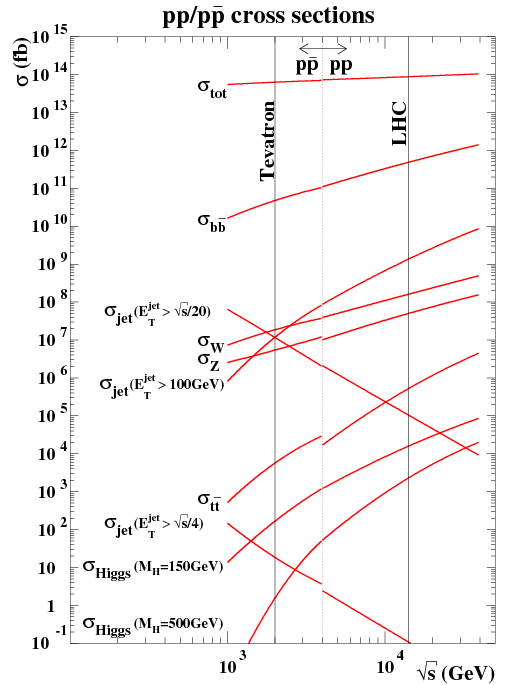
\includegraphics[width=0.43\textwidth]{sec1_cross_lhc.png}
\caption{\label{fig:sec1_cross_lhc}Production cross-sections for several representative processes at hadron colliders. (After~\cite{Weiglein:2004hn})}
\end{figure}

As already mentioned in Chapter~\ref{chap:context}
the ATLAS and CMS collaborations have both observed a particle (with mass $\sim$~125~GeV) 
compatible with the SM Higgs boson in 2012; 
since then the nature of that particle and its coupling to fundamental SM bosons and fermions 
keep being pursued.  Recently ATLAS reported evidence of the $H\to\b\b$ decay~\cite{ATLASHbb2017} 
when it is produced in association with a $W$ or $Z$ boson; the CMS collaboration announced 
the first observation (by a single experiment)
 of Higgs boson decays to $\tau$ leptons~\cite{CMSHtautau2017}. 
The search for the Higgs boson decaying to second generation fermions is next on the 
agenda of the ATLAS and CMS collaborations (see for instance~\cite{ATLASHmumu2017}).

Other than the study of the Higgs boson,
 a central goal of the physics program of the LHC is the exploration of particles and 
interactions at the TeV energy scale, which may hold answers to some of the most profound questions in 
particle physics, like what is dark matter made of and how the Higgs boson mass gets stabilised.

The total delivered luminosity so far from the LHC to the ATLAS experiment  is shown in 
Figure~\ref{fig:intlumivsyear}~\cite{ATLASLumi}.

\begin{figure}[!htpb]
\centering
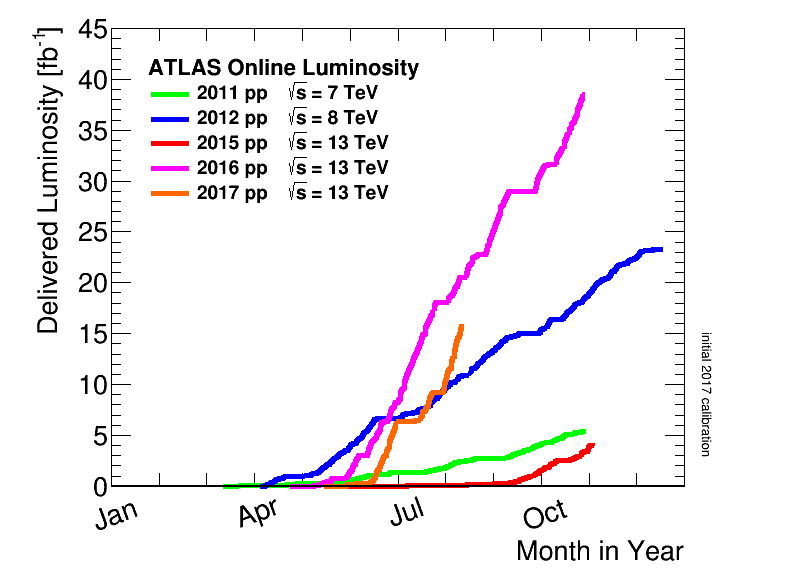
\includegraphics[width=0.62\textwidth]{intlumivsyear.png}
\caption{\label{fig:intlumivsyear}Cumulative luminosity versus day delivered to ATLAS during stable 
beams and for high energy $pp$ collisions. (After~\cite{ATLASLumi})}
\end{figure}

To exploit at best this dataset, to perform precision measurements 
and to face the high interaction rates, radiation doses, particle multiplicities and energies of the
LHC $pp$ collisions the ATLAS detector was built. In the next Section the salient features of this 
detector will be presented.

\section{The ATLAS Detector}
\label{sec:ATLASDetector}
ATLAS~\cite{AtlasDetector} is a general-purpose particle detector covering nearly the entire solid 
angle\footnote{ATLAS uses a right-handed coordinate system with its origin at the nominal interaction 
point (IP) in the centre of the detector and the $z$-axis coinciding with the axis of the beam pipe.  The 
$x$-axis points from the IP towards the centre of the LHC ring, and the $y$-axis points upward. 
Cylindrical coordinates ($r$,$\phi$) are used in the transverse plane, $\phi$ being the azimuthal angle 
around the $z$-axis. The pseudorapidity is defined in terms of the polar angle $\theta$ as $\eta = - \ln 
\tan(\theta/2)$. The distance in ($\eta$,$\phi$) coordinates, $\Delta R = \sqrt{(\Delta\phi)^2+
(\Delta\eta)^2}$, is also used to define cone sizes. Transverse momentum and energy are defined as $
\pt=p\sin\theta$ and $\et=E\sin\theta$, respectively.} around the collision point. It consists of an inner 
tracking detector surrounded by a thin superconducting solenoid, electromagnetic and hadronic 
calorimeters,
and a muon spectrometer incorporating three large superconducting toroidal magnets. 
Figure~\ref{fig:ATLASDetector} shows a schematic view of the ATLAS detector.

\begin{figure}[!htpb]
\centering
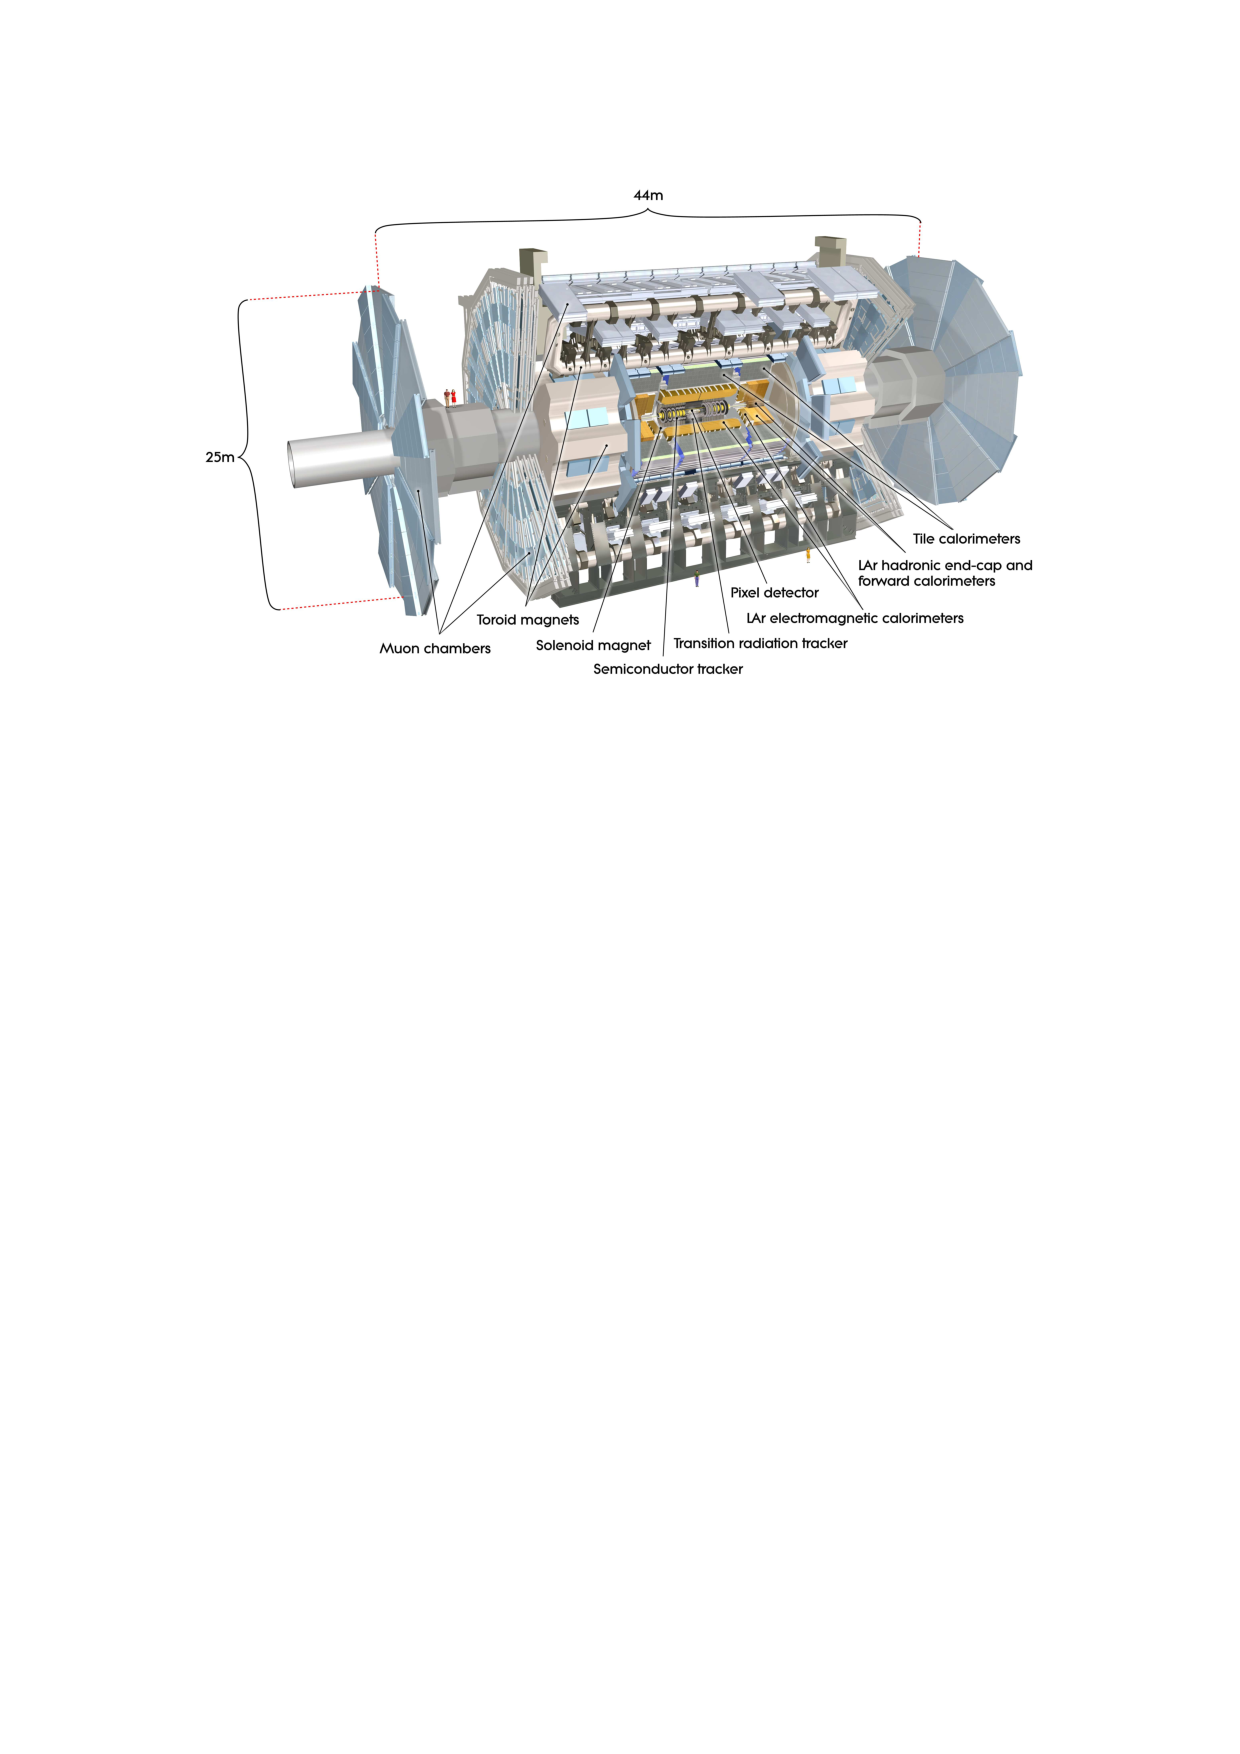
\includegraphics[width=0.65\textwidth]{ATLASDetector.pdf}
\caption{\label{fig:ATLASDetector}Cut-away view of the ATLAS detector. The dimensions of the detector are 25 m in height and 44 m in length. The overall weight of the detector is approximately 7000 tonnes.
 (After~\cite{AtlasDetector})}
\end{figure}


The inner tracking detector (ID or {\it inner detector})~\cite{ATLASIDTDR}, located within a 2~T axial magnetic field generated by the superconducting solenoid, is used to measure the trajectories and momenta of charged particles. The inner layers, consisting of high-granularity silicon pixel detectors, instrument a pseudorapidity
range $|\eta| < 2.5$.
A new innermost silicon pixel layer, the insertable B-layer~\cite{IBLTDR} (IBL), was added to the detector between the first two LHC runs (Run~1 and Run~2 - see Figure~\ref{fig:HL-LHC-plan-2016-01}). The IBL improves the ability to identify displaced vertices and thereby significantly improves the $b$-tagging performance~\cite{ATL-PHYS-PUB-2015-022}. More details 
on the pixel detector will be given in the next Section.
Silicon strip detectors covering $|\eta| < 2.5$ are located beyond the pixel detectors. 
Outside the strip detectors and covering $|\eta | < 2.0$, there are straw-tube tracking detectors, which also provide measurements of transition radiation that are used in electron identification; the so-called 
Transition Radiation Tracker (TRT).
Figure~\ref{fig:ATLASID} shows the barrel section of the ID.

\begin{figure}[!htbp]
\centering
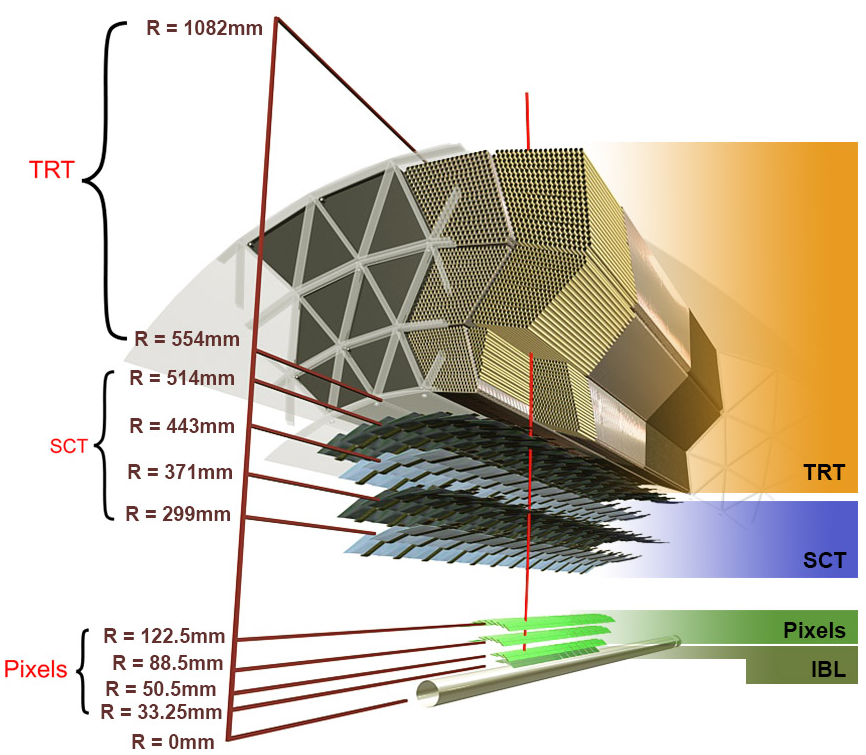
\includegraphics[width=0.65\textwidth]{ATLAS_ID.png}
\caption{\label{fig:ATLASID}Schematic view of the  barrel part of the ATLAS Inner Detector (ID), including the new Insertable B-Layer (IBL). (After~\cite{Potamianos:2016ptf})}
\end{figure}


The calorimeter system covers the pseudorapidity range $|\eta| < 4.9$.
Within the region $|\eta|< 3.2$, electromagnetic calorimetry is provided by barrel ($|\eta| < 1.475$) and
endcap ($1.375 < |\eta| < 3.2$) high-granularity lead/liquid-argon (LAr) electromagnetic calorimeters,
with an additional thin LAr presampler covering $|\eta| < 1.8$ to correct for energy loss in material upstream of the calorimeters.
Hadronic calorimetry is provided by a steel/scintillator-tile calorimeter, segmented into three barrel structures within $|\eta| < 1.7$, and two copper/LAr hadronic endcap calorimeters extend the coverage to $|\eta|=3.2$.
The solid angle coverage for $|\eta|$ between 3.2 and 4.9 is completed with copper/LAr and tungsten/LAr calorimeter modules optimised for electromagnetic and hadronic measurements, respectively.

The outermost part of the detector is the muon spectrometer, which measures the curved trajectories of muons in the field of three large air-core toroidal magnets. High-precision tracking is performed within the range $|\eta| < 2.7$ and there are chambers for fast triggering within the range $|\eta| < 2.4$.

The proton-proton interaction rate at the design luminosity of $L=1.0\times10^{34}$/cm$^{2}$/s 
is approximately 1 GHz, while the event data recording, based on technology and resource limitations, 
is limited to about 1~kHz. For this purpose ATLAS designed 
a  two-level trigger system selects events to be recorded for offline analysis, to assure 
an overall rejection factor of $5\times10^{6}$ against minimum-bias processes while maintaining 
maximum efficiency for the new physics. 
The Level-1 (L1) trigger system uses a subset of the total detector information to make a decision on 
whether or not to continue processing an event, reducing the data rate to approximately 100~kHz between. 
The subsequent  level is a software-based high-level trigger that 
 provides 
the reduction to a final data-taking rate of approximately 1~kHz~\cite{AtlasTrigger2015}. A new Fast TracKer (FTK) system~\cite{FTKTDR} will 
provide global ID track reconstruction at the L1 trigger rate
using lookup tables stored in custom associative memory chips for the pattern recognition.  This 
system is currently being installed and expected to
be fully commissioned by the end of 2017.



\section{The ATLAS Pixel Detector and the Insertable B Layer}
\label{sec:ATLASPixelDetector}

This Section is devoted to the silicon pixel tracking system for the ATLAS experiment. 
The pixel detector was initially composed of three barrel layers plus  a total of six disk layers, three at 
each end of the barrel region~\cite{AtlasPixels}. During the Long Shutdown 1 (LS1), between 
the LHC Run~1 and Run~2 (see Figure~\ref{fig:HL-LHC-plan-2016-01}), a fourth barrel layer was inserted, at a smaller radius than the existing 
pixel detector; it is called the Insertable B-Layer (IBL)~\cite{IBLTDR}.
Figure~\ref{fig:ATLASPixels} shows a schematic view of the ATLAS pixel detector in Run~2; the total 
detector length is 1442~mm. 
\begin{figure}[!htbp]
\centering
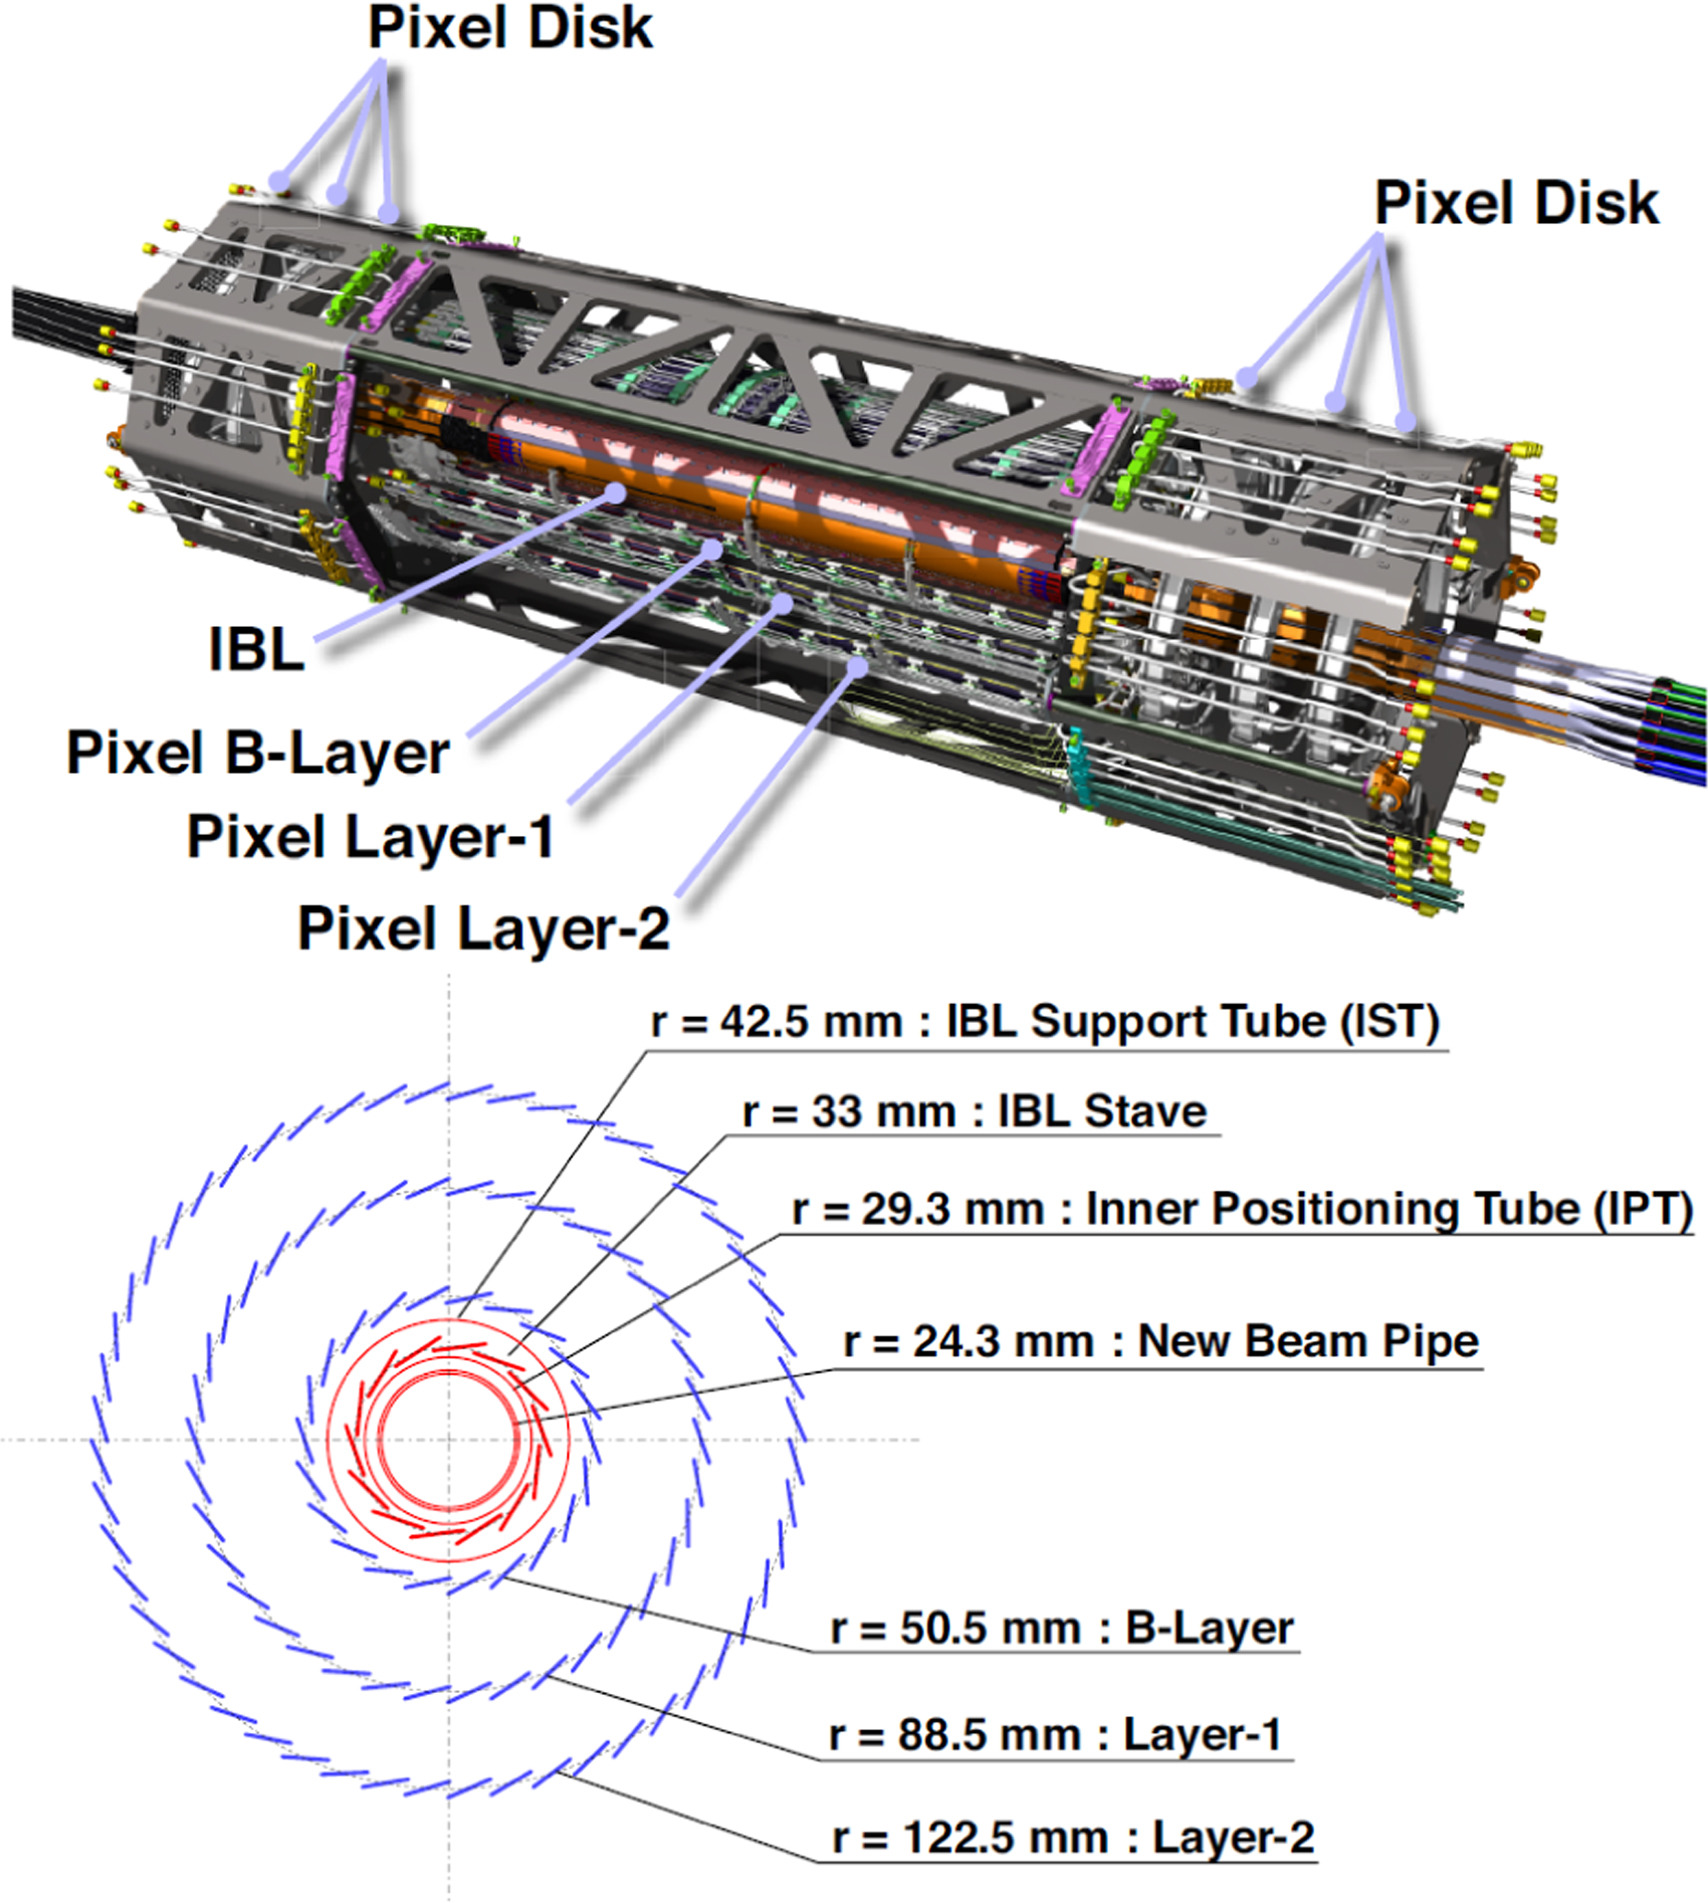
\includegraphics[width=0.65\textwidth]{ATLASPixels.jpg}
\caption{\label{fig:ATLASPixels}Schematic view of the ATLAS 4-Layer Pixel Detector for Run 2. 
On top the different pixel layers are indicated; at the bottom the radii of the four barrel layers are shown, together with the distance from the interaction point of the beam pipe and support structures. (After~\cite{BACKHAUS201665})}
\end{figure}

This Section will cover first the physics motivations and the salient features of the original pixel detector, and later discuss the IBL. The material presented here is taken from~\cite{AtlasPixels,IBLTDR}.

\subsection{Performance Requirements for the Pixel Detector and System Overview}
\label{sec:pixeloverview}
The pixel detector system is the innermost element of the ATLAS ID. The pixel detector contains 
more than 80 million channels and provides pattern recognition capability in order to meet the track 
reconstruction requirements of ATLAS at the full luminosity of the LHC ($L=1.0\times10^{34}$/cm$^{2}$/s). It is the most important detector used in the identification and reconstruction of secondary vertices from the decay of, for example, particles containing a $b$-quark or for $b$-tagging of jets. In addition, it provides excellent spatial resolution for reconstructing primary vertices coming from the $pp$ interaction region within ATLAS even in the presence of the multiple interactions at the LHC design luminosity. 

In what follows the  performance requirements for the pixel detector will be presented, then 
an overview of the system.

\subsubsection{Pixel Detector Performance Requirements}
The performance requirements that guided the design of the pixel detector are:

\begin{itemize}
\item coverage of the pseudorapidity range $|\eta|<2.5$;
\item impact parameter resolution in the transverse plane better than 15~$\mu$m;
\item uncertainty in the longitudinal plane $\sigma(z)$ on the reconstruction of vertices of about 1~mm;
\item three-dimensional-vertexing capabilities;
\item very good b-jet tagging capabilities both in the high-level trigger and in the offline reconstruction; 
\item  minimal material for all elements in the system, in order to reduce multiple scattering and secondary interactions;
\item excellent efficiency for all pixel layers; and
\item radiation hardness of the pixel detectors elements to operate after a total dose of 500 kGy 
and fluence $\Phi=1\times10^{15}$~n$_{\rm eq}$/cm$^2$
\end{itemize}

These performance requirements lead to the following major design choices:

\begin{itemize}
\item three pixel hits over the full rapidity range;
\item minimal radius of the innermost layer (b-layer), set at 5 cm due to the practical limitations of clearances around the interaction region beam pipe vacuum system\footnote{this limit was then overcome with the installation of the IBL};
\item the smallest pixel size achievable, which is set to 50~$\mu$m~$\times$~400~$\mu$m by electronics design limitations.
\end{itemize}

\subsubsection{Pixel Detector Overview}
The pixel tracker is designed to provide at least three points on a charged track emanating from the 
collision region in ATLAS. 
The principal components of the pixel tracking system, before adding the IBL, were the following:
\begin{itemize}
\item the active region of the pixel detector, which is composed of three barrel layers and a total of six disk layers, three at each end of the barrel region;
\item internal services (power, monitoring, optical input/output and cooling) and their associated mechanical support structures (also supporting the interaction region beam pipe) on both ends of the active detector region;
\item a Pixel Support Tube into which the active part of the pixel detector and the services and related support structures are inserted and located; and
\item external services that are connected to the internal services at the end of the Pixel Support Tube.
\end{itemize}

The active part of the pixel system consists of three barrel layers-Layer 0 (so-called b-layer), Layer 1 
and Layer 2-and two identical endcap regions, each with three disk layers, as it cam be seen in 
Figure~\ref{fig:ATLASPixels}. The basic building block of the active part of the pixel detector is a module 
that is composed of silicon sensors, front-end electronics and flex-hybrids with control circuits.
Modules are mounted on mechanical/cooling supports, called staves, in the barrel region. 
In the endcap modules are mounted on mechanical/cooling supports, called disk sectors; There are 
eight identical sectors in each disk. The concept of  pixel module is illustrated in Figure~\ref{fig:Pixel_module}.
\begin{figure}[!htbp]
\centering
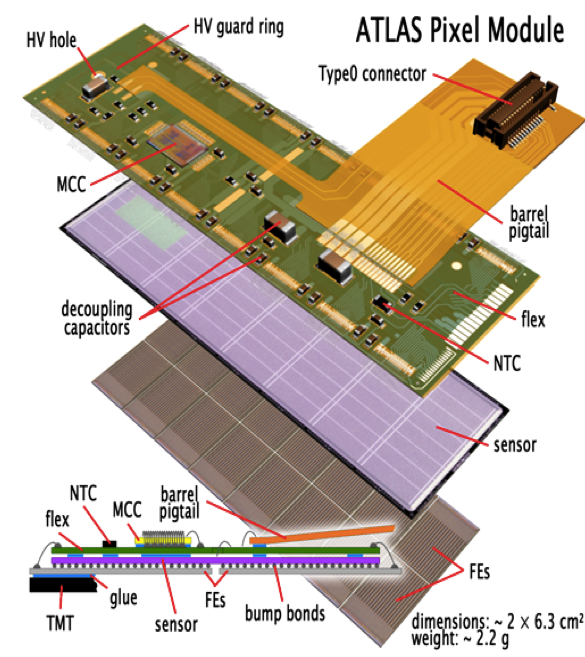
\includegraphics[width=0.65\textwidth]{Pixel_module.png}
\caption{\label{fig:Pixel_module}Assembly view and cross-section of an ATLAS Pixel Detector module. (After~\cite{AtlasPixels})}
\end{figure}


A description of the pixel sensors and electronics characteristics follows.

\subsubsection{Pixel Sensors}
\label{sec:pixelsensors}

The total number of pixels in the system is approximately 67 million in the barrel and 13 million in the endcaps, covering a total active area of about 1.7~m$^2$.
The  sensors  choice for ATLAS was of $n-on-n$ pixels on high resistivity, nominally 250~$\mu$m 
thick bulk. For each sensor tile, the 47232 pixel implants are arranged in 144 columns and 328 rows. 
For most of the pixel cells the pitch is of 	400~$\mu$m~$\times$~50~$\mu$m; in 16 columns 
the pitch is of 600~$\mu$m~$\times$~50~$\mu$m. In each column eight pairs of pixel implants, located 
near the center lines, are ganged to a common read-out, resulting in 320 independent read-out rows or 
46080 pixel read-out channels. This arrangement was chosen to allow for the connection of the sensor 
tile to 16 electronic front- end chips (see next Section). 
Oxygen impurities had been introduced in the bulk to increase tolerance of the silicon against bulk damage caused by charged hadrons~\cite{Lindstrom:421210,LINDSTROM200160}.
The sensors can be fully depleted before type inversion with bias voltages below 100~V. After type 
inversion the depletion zone grows primarily from the segmented $n^+$ implant when the region of 
highest electric field in the bulk now converts to $p$-type.

On the sensor front side, pixel structures are arranged and isolated by moderated p-spray impants, 
which have proven to be radiation tolerant with respect to surface damages induced by ionising charged 
particles for doses up to 500~kGy in silicon. The layout of the moderated p-spray impants is 
shown in Figure~\ref{fig:modpspray}. This isolation technique avoids high field regions in the interface between the pixel isolation and the bulk and ensures radiation tolerance of the design.
\begin{figure}[!htbp]
\centering
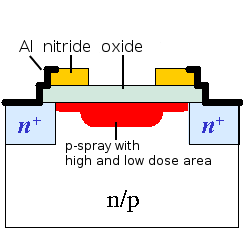
\includegraphics[width=0.49\textwidth]{modpspray.png}
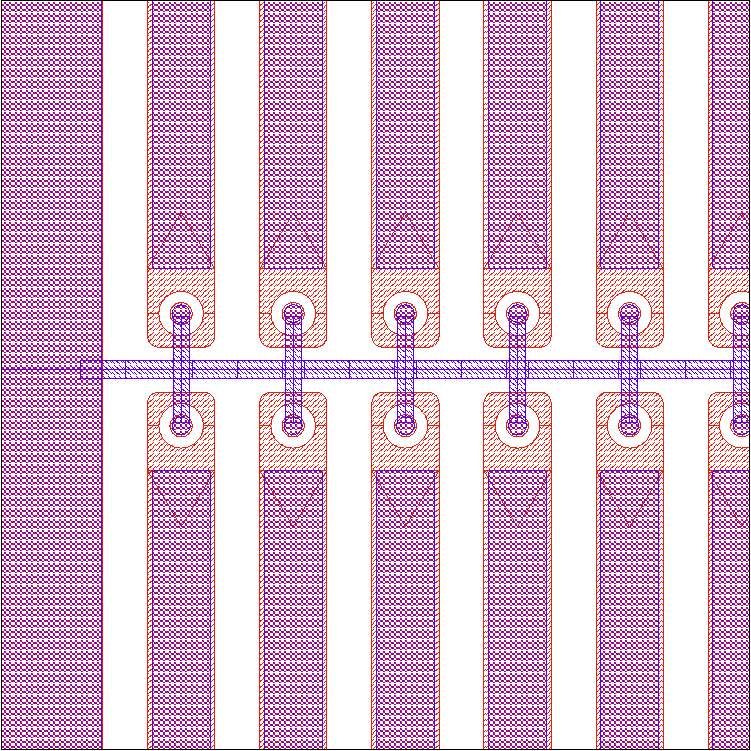
\includegraphics[width=0.39\textwidth]{biasgrid.png}
\caption{\label{fig:modpspray}(left) Layout of the moderated p-spray isolation. (right)  Layout detail of the bias grid (After~\cite{AtlasPixels})}
\end{figure}
All 46080 read-out channels of a sensor tile are connected to a common bias grid structure, presented 
in Figure~\ref{fig:modpspray}, by employing a punch-through connection technique to each channel.
 The method biases the entire sensor without requiring individual connections, but still ensures isolation between pixels. The bias grid has been used for quality assurance measurements before the read-out electronics are connected to the sensors. 

On the sensor tile backside a series of guard rings (GRs) were defined by $p^+$ implants. The GRs 
assures a controlled potential drop from  $p^+$ implant negative bias voltage to ground. 
A sketch of the pixel sensor edge, with the read out electronics on top is given in 
Figure~\ref{fig:sensorbb}.
\begin{figure}[!htbp]
\centering
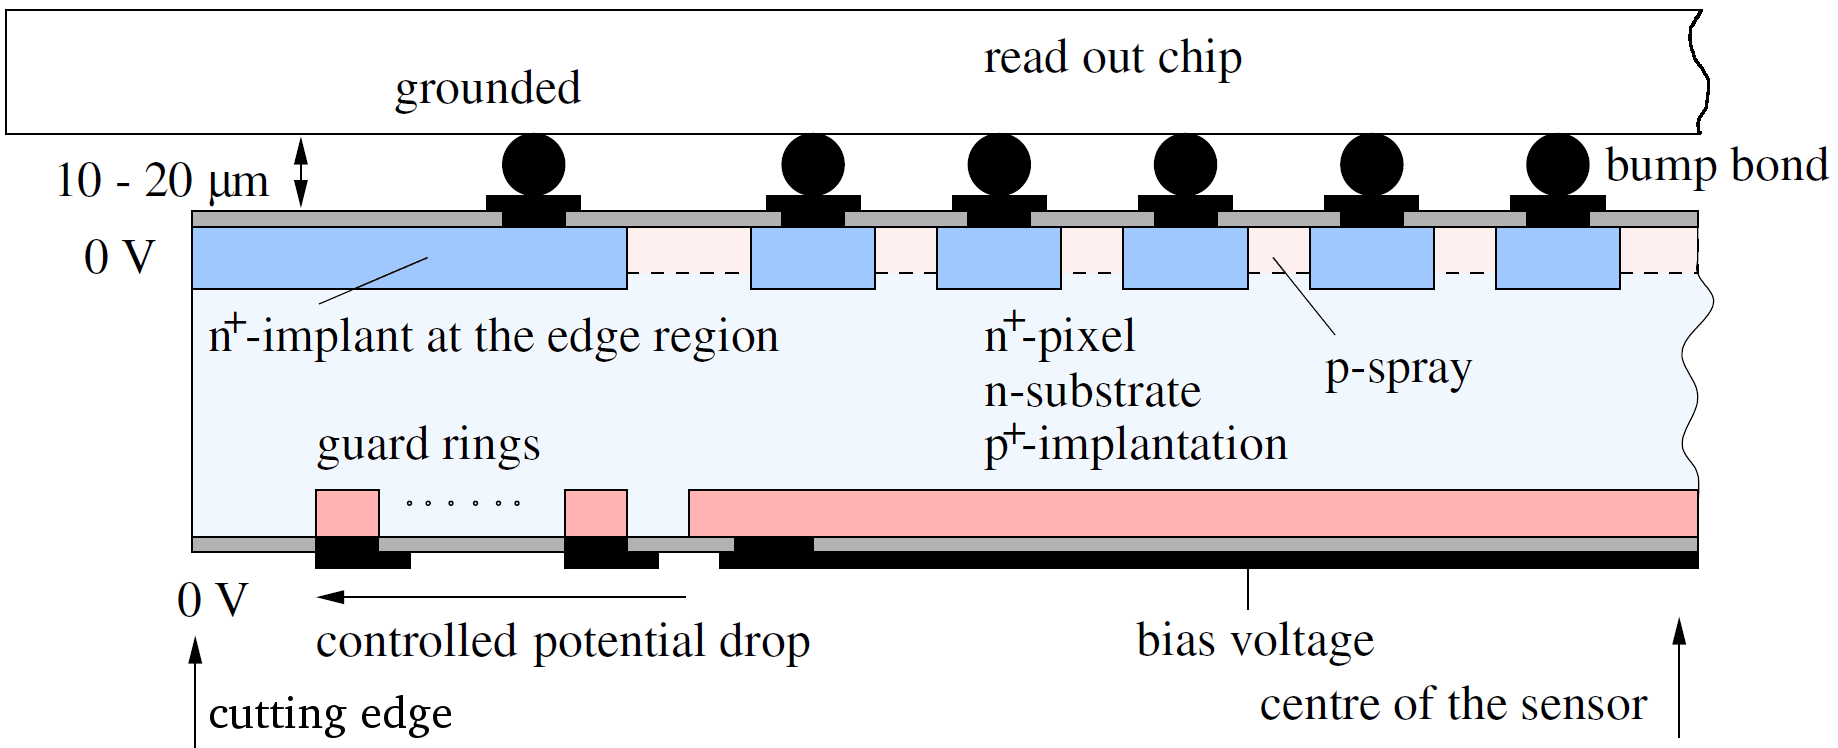
\includegraphics[width=0.65\textwidth]{sensorbb.png}
\caption{\label{fig:sensorbb} Cross section sketch of the ATLAS pixel module (After~\cite{Altenheiner:2012zz})}
\end{figure}

\subsubsection{Pixel Electronics}
\label{sec:pixelel}
A block diagram that illustrates the principal elements of the system architecture of pixel 
electronics is shown in~\ref{fig:pixelel}.

\begin{figure}[!htbp]
\centering
\includegraphics[width=0.65\textwidth]{pixelel.png}
\caption{\label{fig:pixelel}Block diagram of the pixel detector system architecture. (After~\cite{AtlasPixels})}
\end{figure}
There are 16 FEI3~\cite{FEI3} front-end chips (FE) in each pixel module and these are arranged in two rows of eight chips. 
The readout chip for the ATLAS pixel detector contains 2880 pixel cells of 400~$\times$~50~$\mu$m$^2$ size arranged in an 18$\times$160 matrix. Each pixel cell contains 
an analogue block where the sensor charge signal is amplified and compared to a programmable
threshold using a comparator. The digital readout part transfers the hit pixel address,
a hit leading edge (LE) timestamp, and a trailing edge (TE) timestamp to the buffers at the chip
periphery. In these buffers a Time-over-Threshold (ToT) is calculated by subtracting the TE from
the LE timestamp. Hits marked by trigger signals are
selected for readout. Triggered hit data are then transmitted serially out of the chip in the same
order as the trigger arrival.
 The duration of the ToT is measured by counting the cycles of the 40~MHz master chip
clock. Due to the pulse shape of
the preamplifier the ToT is a nearly linear function of the deposited charge. 
Evaluating this ToT
information can therefore be used to infer the charge deposi
ted by a passing particle.  The ToT  mechanism is presented in Figure~\ref{fig:tot}.

\begin{figure}[!htbp]
\centering
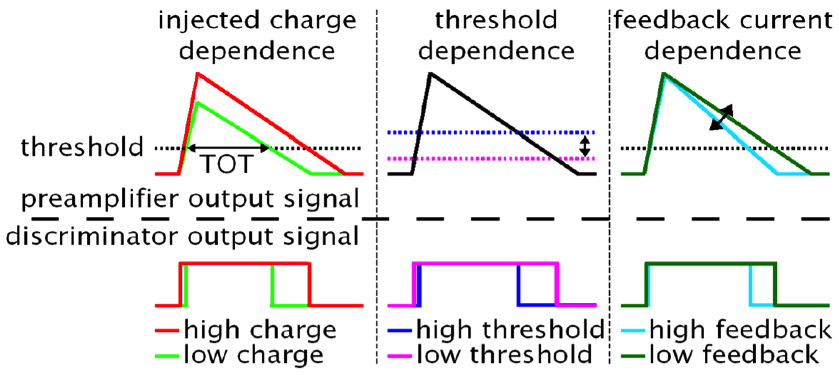
\includegraphics[width=0.65\textwidth]{tot.png}
\caption{\label{fig:tot} (left)Time-over-Threshold mechanism (ToT) and its dependence on the injected charge; (center) ToT dependence on threshold value; (right) ToT dependence on feedback current.
 (top) Shaper output; (bottom) discriminator output. (After~\cite{AtlasVertexing2009})}
\end{figure}

The 16 FEs are read out by a Module Control Chip (MCC). Each module is then connected to the off-
detector Read-out Drivers (RODs) through optical-fiber links (opto-links).
One down link is used to transmit
clock, trigger, commands and configuration data, while one or two up-links are used for event
readout.
The readout (R/O) architecture is ``datapush''.
This means that each component in the chain (FE, MCC) always transmits at the maximum
rate, and there is no busy mechanism to stop transmission when buffers are full. 

%The power supply system uses a combination of customized-commercial components and
%fully-custom components for the low (electronics) and high (sensor bias) voltages.
%The optical-links are custom made using commercial diode and laser array bare die with custom integrated circuits (DORIC and VDC) and packaging. An optical-interface card (Back of Crate or BOC) is also used for each ROD.

\subsubsection{Pixel Support and Services}
\label{sec:pixelservices}

As already mentioned in the system overview, the pixel system consists of three barrel layers and two identical endcap regions, each with three disk layers. Figure~\ref{fig:pixstruc} shows the salient 
features of the pixel structure.

\begin{figure}[!htpb]
\centering
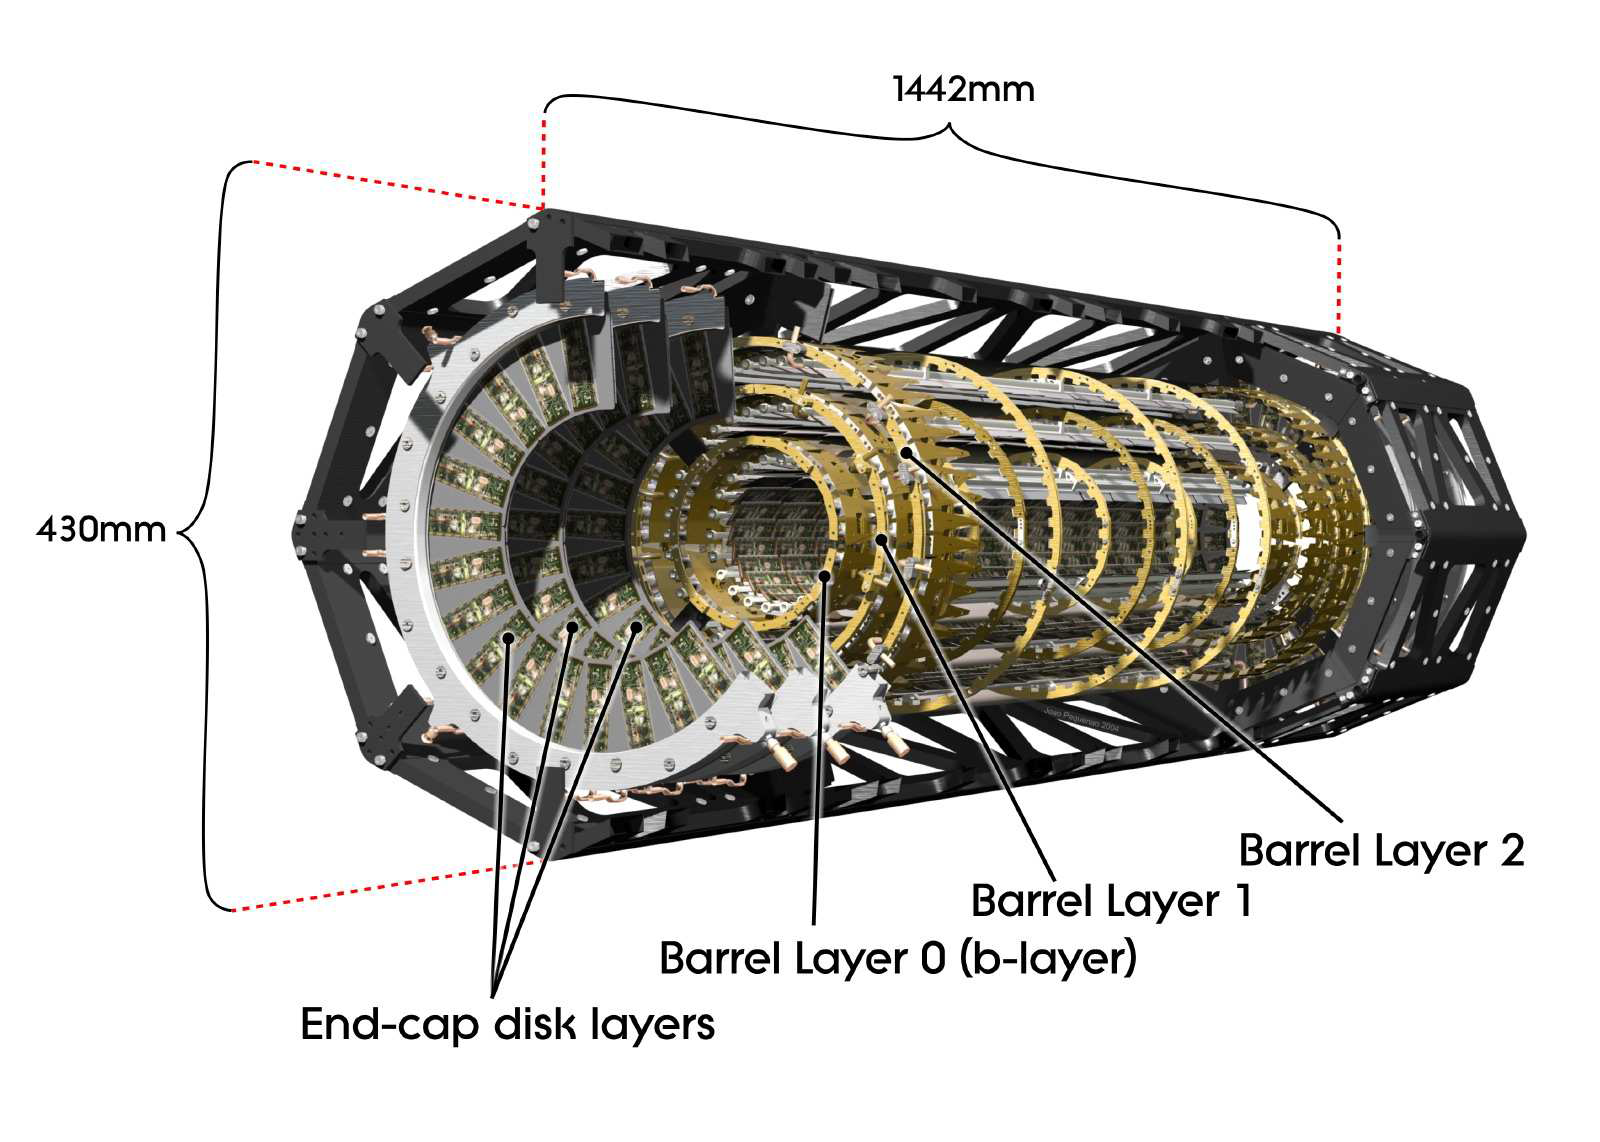
\includegraphics[width=0.65\textwidth]{pixstruc.png}
\caption{\label{fig:pixstruc} A schematic view of the active region of the pixel detector consisting of barrel and endcap layers. (After~\cite{AtlasPixels})}
\end{figure}

Modules are mounted on mechanical/cooling supports, called staves, in the barrel region. Thirteen 
modules are mounted on a stave and the stave layout is identical for all layers. The active length of 
each barrel stave is about 801 mm. The staves are mounted in half-shells manufactured from a carbon-
fiber composite material. Two half-shells are joined to form each barrel layer.
The two endcap regions are identical. Each is composed of three disk layers, and each disk layer is 
identical. Modules are mounted on mechanical/cooling supports, called disk sectors. There are eight 
identical sectors in each disk.

The barrel shells and the endcap disks are supported by a spaceframe also manufactured from a 
carbon-fiber composite material (see Figure~\ref{fig:pixstruc}). Electrical, optical and cooling services 
are con- nected and routed within service panels (four on each end of the pixel detector) from patch 
panels (Patch Panel 0-PP0) at the ends of the supporting spaceframe to the end of the Pixel Support 
Tube.
These services are supported by carbon fiber structures that also hold the beryllium vacuum pipe within 
the Pixel Support Tube. Electrical, optical and cooling connections are made at the end of the Pixel 
Support Tube.

\subsection{Performance Requirements for the IBL and System Overview}
\label{sec:IBLoverview}

The Insertable B-Layer (IBL) is a fourth layer added to the present Pixel detector between a
new beam pipe and the pixel B-layer. The principal motivations for the IBL were:

\begin{itemize}
\item tracking robustness, to cope with predicted failures of the pixel layers, in particular the B-layer; 
  a loss of data in the B-layer
seriously deteriorates the impact parameter resolution, directly affecting the $b$-tagging. The
IBL restores the full $b$-tagging efficiency even in case of a complete B-layer failure.
  \item Coping with luminosity effects, like increased event pile-up which leads to  high occupancy that can induce readout inefficiencies. The presence of event pile-up requires redundancy in
the measurement of tracks in order to control the fake rate arising from random combinations
of clusters in events with high pile-up background. The addition of the IBL layer, with
comparably low occupancy, helps to preserve tracking performance in face of luminosity
effects.
  \item Tracking precision: The IBL located close to the interaction point improves the quality of
impact parameter reconstruction for tracks, and thereby improves vertexing and b tagging
performance. As a result, sensitivity for signals in physics channels involving $b$ jets is improved,
for instance for a low mass SM Higgs in the channel $WH,\,H\to b\bbar$.
\end{itemize}

Strong constraints and project specifications had a substantial impact on the technologies
required for the IBL:

\begin{itemize}
\item the smaller radius of the IBL required development of a more radiation hard technology for
sensors and electronics.
\item The small radius between the new beam pipe needed to be able to insert the IBL
 and the existing pixel detector does not allow
for tilting of modules in the longitudinal direction (along the beam). Sensors with either
an active edge or a slim guard ring must therefore be developed to reduce geometrical inefficiencies.
Full coverage in $\phi$ is possible by constructing modules with the same active
width, but with only one row of front-end chips. The new front-end chip has five times the
area of the chip in the existing pixel detector and covers an active area that is 90\% of the
sensor. (The active fraction of the present pixel modules is 75\%.)
 \item Minimizing material is very important in the optimization of tracking and vertexing performance.
The IBL radiation length will represent just 60\% of the pixel B-layer. Low
radiation length was achieved by considering more aggressive technology solutions, in addition
to new module design, technologies such as: local support structures (staves) made of low
density carbon foams; CO$_2$ evaporative cooling, which is more efficient in term of mass flow
and pipe size.
\end{itemize}

The IBL modules are supported by means of fourteen local supports, the Staves, arranged cylindrically
around the beam pipe. Some overlap between modules is provided by tilting each stave
about 14$^{\circ}$. The nominal layer radius, that is the distance from the beam axis to the sensor's
centre-of-mass, is $R$ = 33.25~mm. The $r\phi$ view of the IBL layout is shown in Figure~\ref{fig:IBLrphi}. The stave is $L$ = 724~mm long. The IBL was successfully installed in May 2014.


\begin{figure}[!htpb]
\centering
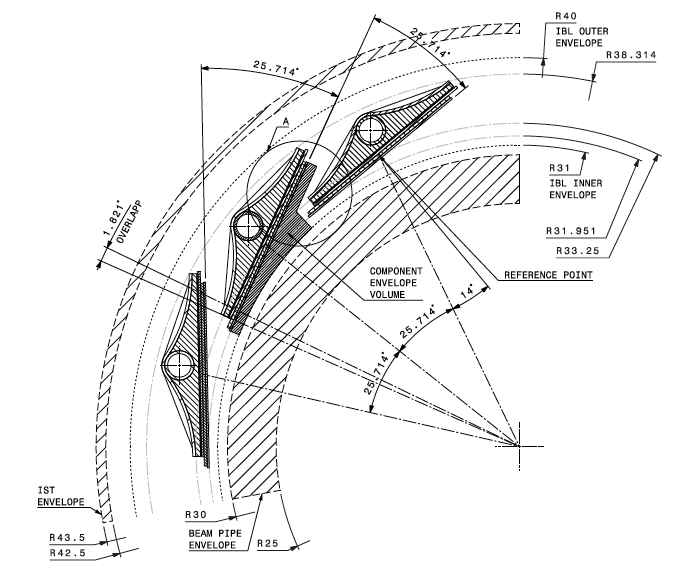
\includegraphics[width=0.65\textwidth]{IBLrphi.png}
\caption{\label{fig:IBLrphi}IBL layout: $r\phi$ view. (After~\cite{IBLTDR})}
\end{figure}

\subsubsection{IBL Pixel sensors}
Two sensor technologies are used in the IBL: planar $n-on-n$ sensors of the same type
that was used for the pixel detector, and 3D sensors, which are a 
technology that has not
been used in a HEP experiment before. In 3D sensors the electrodes are columns in
the silicon~\cite{PARKER1997328}. There can be varying numbers of electrodes per pixel which will 
have an influence on charge collection and noise; for IBL a design with two electrodes per pixel was chosen. A schematic view of the 3D sensors is shown in Figure~\ref{fig:IBLtredi}.
\begin{figure}[!htpb]
\centering
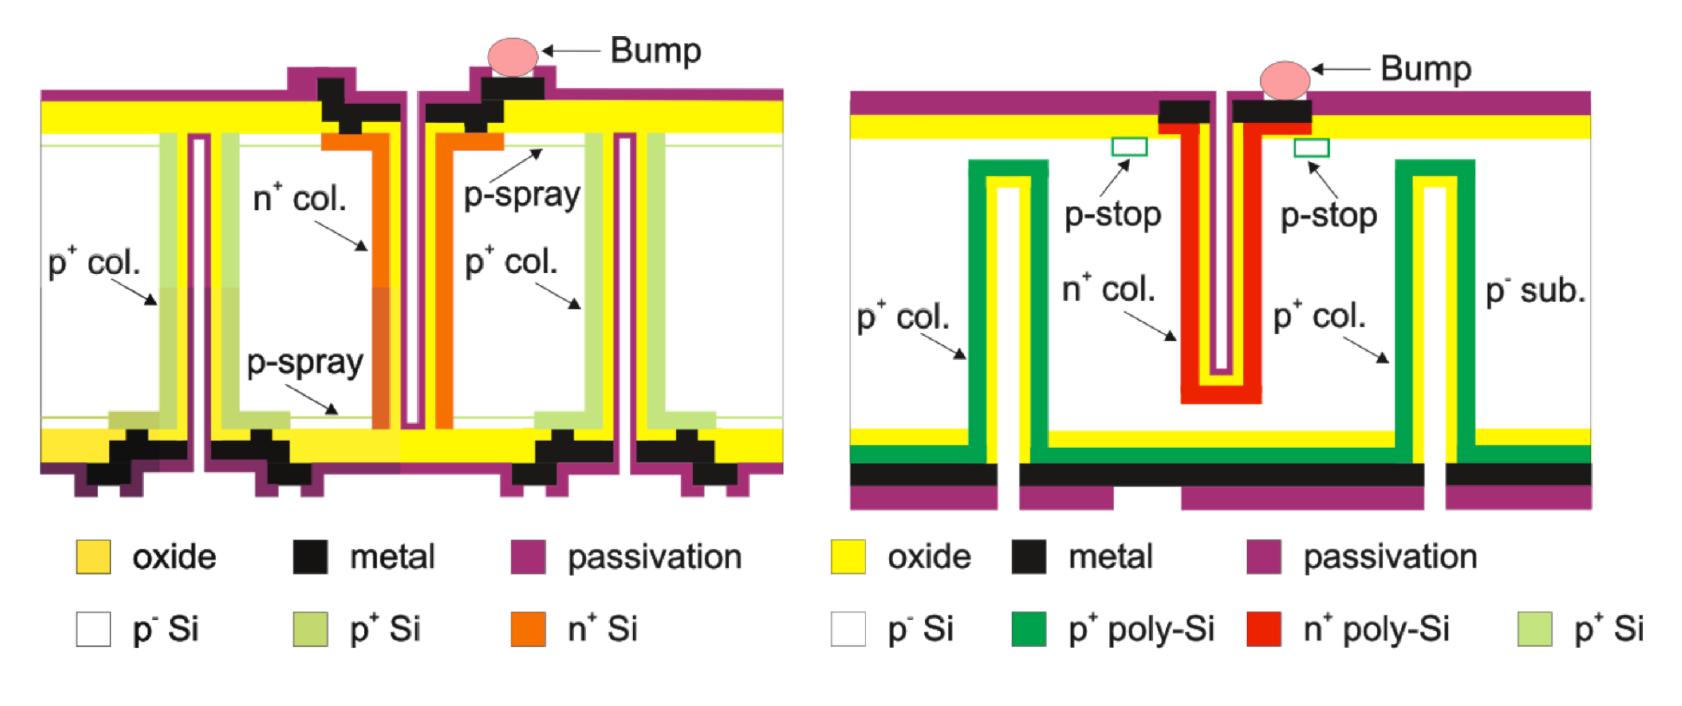
\includegraphics[width=1.00\textwidth]{tredi.png}
\caption{\label{fig:IBLtredi} Schematic cross-section of the 3D detector with passing-through columns from FBK (left) and
with partial columns from CNM (right) fabricated on a $p-$type substrate (not to scale)(After~\cite{Darbo:2014kma})}
\end{figure}



\begin{table}[!htpb]
\caption{\label{tab:IBLsensors}Comparison of parameters between planar and 3D IBL sensors.}
\centering
\begin{tabular}{rll}
\hline
 & Planar & 3D\\
 \hline
 \hline
 Vendor & CiS & FBK/CNM \\
 Wafer Thickness & 200~$\mu$m & 230~$\mu$m \\
 Size in FE chips & 2 & 1\\
 Depletion voltage before irradiation & 35-50~V & 15~V \\
 Depletion voltage at the end of the life & 1000~V & 180~V\\
 \hline
 \end{tabular}
\end{table}
The properties of the sensors are summarised in Table~\ref{tab:IBLsensors}.
Pixel pitch is 50~$\mu$m~$\times$~250~$\mu$m for both technologies. 
Both sensor types have a slim edge of 200~$\mu$ which is needed to avoid gaps in the coverage in $z$ since shingling of the sensors in $z$ is not possible for IBL. 
To reduce the area at the detector edge to 200~$\mu$, with respect to 1.1~mm for pixel modules, 
two strategies were implemented: planar ``moved'' GRs inward, inside the area defined by $n^+$ 
pixel implants (see also Figure~\ref{fig:IBLSlimEdge});  3D sensors has a forest of $p^+$ columns 
at bias voltage; in addition to that CNM sensor had a fence of $n^+$ columns shorted together to form a GR.
\begin{figure}[!htpb]
\centering
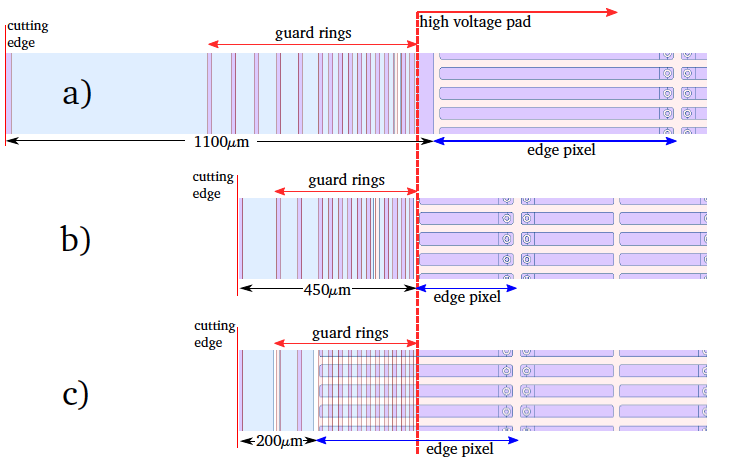
\includegraphics[width=0.65\textwidth]{IBLSlimEdge.png}
\caption{\label{fig:IBLSlimEdge}Top view of the sensor edge region of the ATLAS pixel (a), the conservative(b) and the slim edge (c) IBL design. The $n^+$ implantation is seen in blue the $p^+$ implantation in red. By reducing the number of guard rings, narrowing of the safety margin and by extending the edge pixels beyond the high voltage pad, the inactive edge could be reduced from 1100~$\mu$m for the ATLAS pixel design to 200~$\mu$ for the slim edge IBL design. (After~\cite{WittigPHD})} 
\end{figure}

Instead of choosing one technology over the other it was decided in the end to use a mix of sensors: 75\% planar in the center of each stave, and 25\% 3D on the outsides~\cite{AtlasVertexing2012}.


\subsubsection{IBL Pixel Electronics}

The frontend readout chip for IBL is the FE-I4~\cite{FEI4}. One FEI4 contains 26880 pixels which are arranged in 80 columns in $z$ and 336 rows in $\phi$. The size of one pixel is of course 
250~$\mu$m~$\times$~50~$\mu$m.
A crucial new feature of this chip with respect to the FEI3 readout chip is that the hits are stored in the 
pixel cells. A hit is only read out if a trigger request matches its timestamp, otherwise the hit is deleted. 
This reduces bandwidth use and power consumption inside the chip and allows for far higher 
occupancies.

The chip provides 4-bit ToT information for each hit compared to 8 of FEI3. To reduce data size the data of two neighboring pixels in $\phi$ are sent out in a single data word.

Figure~\ref{fig:TwoFEIs} shows the FEI3 and FEI4 chip side-by-side.
\begin{figure}[!htpb]
\centering
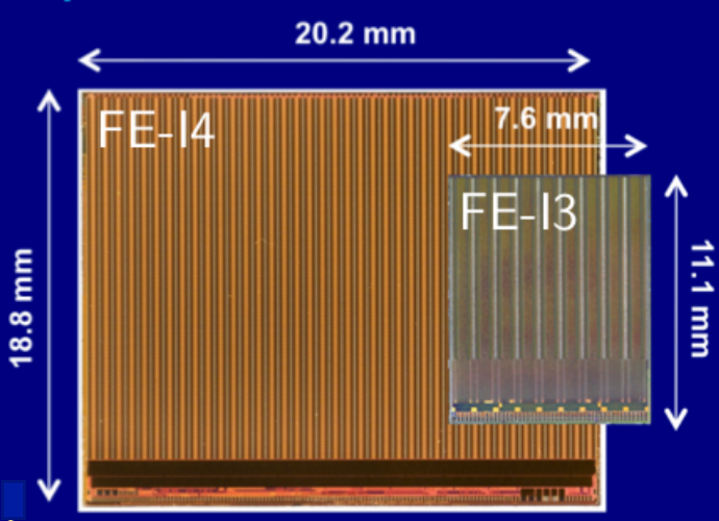
\includegraphics[width=0.65\textwidth]{TwoFEIs.pdf}
\caption{\label{fig:TwoFEIs}FEI3 and FEI4 chip side-by-side. Chips dimensions are indicated.}
\end{figure}

\subsubsection{IBL Structure}
The IBL is composed of 14 staves.
Each stave contains 12 double-chip sensors in planar technology and 8 single-chip sensors in 3D 
technology. The total length of the active area of the save is 640~mm; including stave services it 
extends to 7~m.

The stave design is based on carbon foam material that provides a path for the heat generated in the sensors and in the front-end chips, to the cooling fluid boiling at low temperature in the cooling channel. 
The stiffness of the structure is provided by a quasi-isotropic carbon fiber laminate, the {\it Omega}, that is bonded to the foam. Figure~\ref{fig:Omega} shows the cross section and a 3D view of the stave.

\begin{figure}[!htpb]
\centering
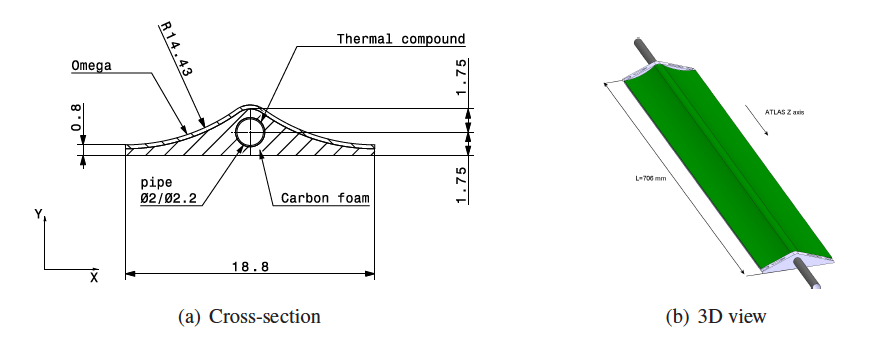
\includegraphics[width=0.65\textwidth]{omega.png}
\caption{\label{fig:Omega}Cross section and 3D model of the IBL stave. Dimensions are in millimeters.
 (After~\cite{IBLTDR})}
\end{figure}

The cooling pipe is sandwiched between the carbon foam and the {\it Omega}. The pipe is hard bonded
to the structure, the thermal contact being provided by a thermal compound based on epoxy-loaded
resins. Inside the pipe $CO_2$ boiling assures the needed evacuation of the power dissipated 
by the IBL pixel modules. The target temperature
for operating the IBL sensors is approximately -15$^{\circ}$C, in order to minimise effects of reverse
annealing on the sensors and to avoid thermal runaway. At the end of their lifetime 
planar sensors are expected to dissipate between 200~and~500~mW/cm$^2$, depending 
on the annealing history. The chip adds another 400~mW/cm$^2$, for a total of slightly less than 
1~W/cm$^2$. After performing thermal simulations it was chosen to set a $CO_2$ evaporation 
temperature of $-40^{\circ}$C and a mass flow per stave in the range of 1.5 to 2 g/s.

\section{Summary}
In this Chapter the ATLAS Pixel detector has been presented, after a review of the physics program 
of the ATLAS experiment. In the next Chapter the radiation damage to the ATLAS pixel sensors 
will be described and a tool to model it will be discussed.

